\newpage
\thispagestyle{sectioned}
\chapter{Tecnologías del Proyecto}
 
\section{Tecnologías de Wave}

  TABLA RESUMEN: Google Wave, Apache Wave, WIAB, SwellRT, GitHub, Java, GWT, JavaScript, HTTP, 
  
  \subsection{Google Wave}

  Ideado y presentado en 2009 por ingenieros de Google \cite{ref:wave_announcement}, Wave es a la vez un protocolo de comunicaciones \cite{ref:wave_over_xmpp} y una plataforma web de código libre, que permiten a sus usuarios comunicarse y colaborar entre sí en tiempo real (Ver sección \ref{sssec:realTime}) y de forma federada (Ver sección \ref{sssec:federation}) a través de Internet. 
  Inicialmente fue desarrollado con el objetivo de integrar en una sola plataforma servicios ampliamente utilizados como son el correo electrónico, las redes sociales y la mensajería instantánea. Pese al gran entusiasmo generado entre la comunidad de desarrolladores tras su anuncio, en el año 2010 Google anuncia el abandono del proyecto \cite{ref:google_wave_end} debido a su poca acogida entre los desarrolladores y a que decide reorientar el uso de la tecnología hacia sus plataformas de edición de documentos Google Docs \cite{ref:google_docs} y a su red social Google + \cite{ref:google_plus}.  Es en este momento cuando el desarrollo libre del proyecto pasa a manos de la Apache Software Foundation bajo el nombre de Apache Wave.

  \subsection{Apache Wave}
  
  Al cambiar de manos su desarrollo en 2010, la tecnología pasa a formar parte de la incubadora de la fundación Apache \cite{ref:apache_wave_about} como software de código libre bajo licencia Apache \cite{ref:apache_license}. Así, se produce el desarrollo de Wave In a Box (WIAB) (Ver sección \ref{sec:wiab}), plataforma que integra un cliente web sencillo y una implementación de un servidor Wave que cualquiera puede descargar y desplegar en su ordenador.
  
  \subsection{Características de Wave}
  
  Como plataforma de código libre desarrollada para ser utilizada en red, Wave hace uso de distintas tecnologías y protocolos bien conocidos. Entre sus características más destacadas están las siguientes:

    \subsubsection{Federación}\label{sssec:federation}
    
    El Protocolo Wave \cite{ref:wave_over_xmpp} fue desarrollado para utilizar un modelo federado \cite{ref:wave_federation} \cite{ref:wave_white_paper} de comunicación basado en la tecnología XMPP \cite{ref:xmpp} \cite{ref:wave_over_xmpp}. Se trata por tanto de un modelo descentralizado en el que cualquiera de los participantes en la conversación es libre de actuar tanto como servidor como cliente sin que ello afecte a su participación en la conversación. 
    Además, a diferencia de otras tecnologías (como el correo electronico) en las que cada participante almacena su propia copia de la conversación y cada vez que hay cambios se debe transmitir la conversación entera a todos los participantes, Wave tiene la ventaja de que actúa de forma que es el servidor de la conversación el único que almacena la copia entera y se encarga de calcular los cambios que se han producido para transmitir solamente dichos cambios por la red a los participantes, con las consiguientes ventajas en términos de latencia que ello conlleva. 

    \subsubsection{Consistencia en tiempo real}\label{sssec:realTime}
    
    El Protocolo Wave \cite{ref:wave_over_xmpp} utiliza la tecnología de Transformaciones Operacionales (OT) \cite{ref:how_ot_works} para garantizar la consistencia en la comunicación en tiempo real entre los participantes. Es decir, cualquier cambio producido por cualquiera de los participantes en la conversación se transmite automáticamente y en tiempo real al resto de los participantes sin pérdida de información y garantizando que los cambios se muestran en el estricto orden en el que se produjeron sin errores \cite{ref:wave_ot}.
    
    \subsubsection{Escalabilidad}
    
    Wave fue desarrollado como un protocolo de alta escalabilidad que permite gestionar la existencia de una gran cantidad de conversaciones y participantes sin que por ello se resienta la productividad del sistema.
    
    \subsection{Servidores Wave}
  
    \subsubsection{Wave in a Box}\label{sssec:wiab}
    
    Wave In a Box (WIAB) \cite{ref:wave_in_a_box} es el nombre de la implementación de un servidor Wave desarrollado por la Apache Software Foundation tras pasar el proyecto a sus manos en el año 2012. Al igual que el resto del código de la tecnología que heredó de Google, está implementado en Java usando OpenJDK \cite{ref:openjdk}. La instalación trae consigo un cliente web desarrollado en Javascript usando el framework Google Web Toolkit \cite{ref:gwt}. Este cliente web sirve como prueba de concepto de las funcionalidades básicas del Modelo Conversacional de Wave, pudiendo gesionar waves, usuarios y extesiones. Actualmente cualquiera puede descargar y desplegar WIAB en su ordenador siguiendo los pasos que nos proporcionan en su wiki \cite{ref:wave_in_a_box_wiki}. La aplicación se distribuye en forma de código fuente, accesible entre otras formas desde su repositorio de GitHub \cite{ref:wave_in_a_box_github}. Existen asimismo servidores de prueba ya desplegados en Internet sobre los que se puede observar el funcionamiento de WIAB \cite{ref:wave_in_a_box_server}.
   
   
    \begin{figure}[H]
      \centering
	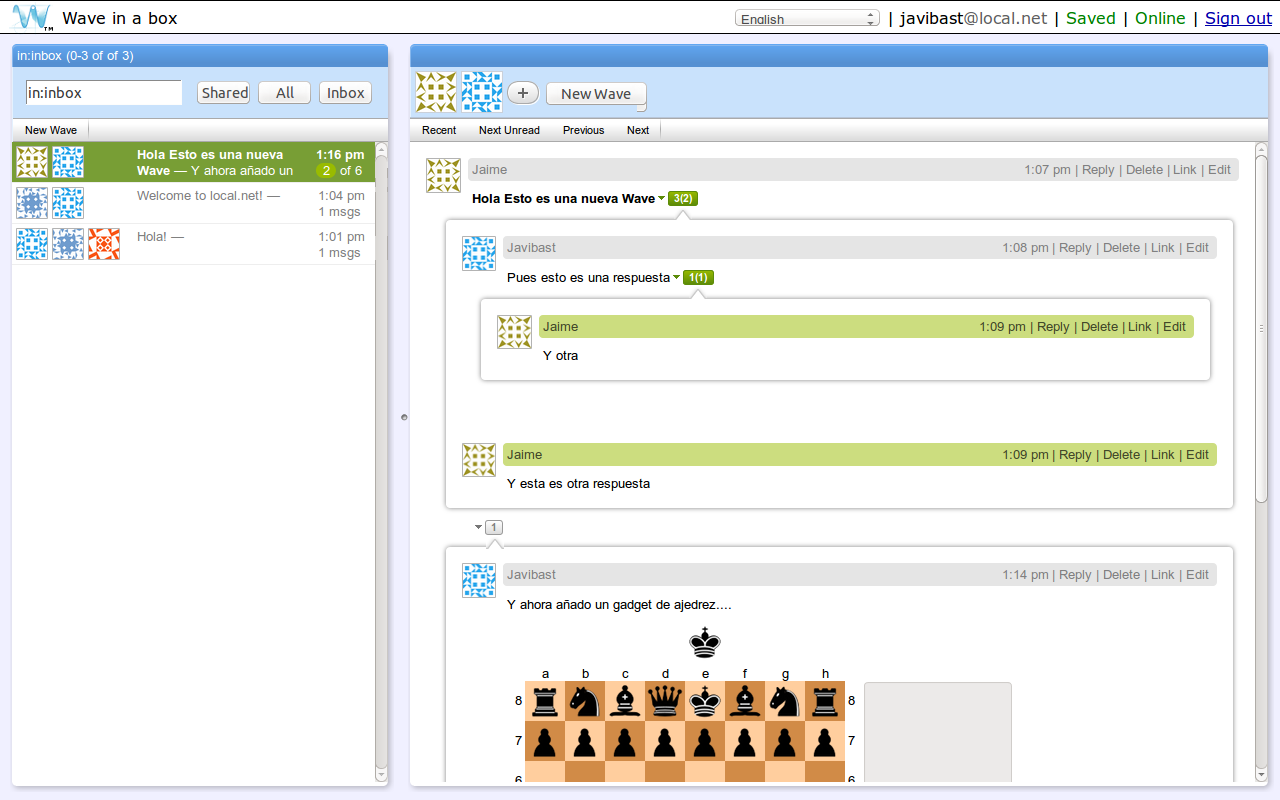
\includegraphics[keepaspectratio, scale=0.3]{Media/Captures/WIAB_Server.png}
      \caption{Cliente Wave In A Box}
      \label{fig:wiab_client}
    \end{figure}
   
    \subsubsection{SwellRT}\label{sssec:swellRT}
    
    Como parte del proyecto europeo P2PValue \cite{ref:p2pvalue} existe SwellRT, un fork de WIAB que amplía las características de éste último añadiendo un nuevo modelo de datos (Modelo de Datos Colaborativo) más allá del Modelo de Datos Conversacional de Wave original. Proporciona también un API escrito en Java que permite trabajar sobre los datos de ese nuevo modelo en forma de tres tipos básicos: mapas, listas y strings. Es por tanto un framework de colaboración en tiempo real que basa su funcionamiento en Apache Wave y cuyo principal popósito es permitir la integracion de la tecnología Wave en otras aplicaciones, que podrán compartir objetos (de los tipos antes mencionados) de forma federada y en tiempo real. Su código fuente está disponible en GitHub \cite{ref:swellRT_github}, así como sus instrucciones de instalación (Ver el Readme en GitHub).\\[.2cm]

    Para este proyecto se ha usado el framework SwellRT como base para la migración de la tecnología de Apache Wave a la plataforma Android \cite{ref:android_platform}. Se pretende con esto que SwellRT haga uso de las funcionalidades nativas de Android.
       

\section{Tecnologías de la Aplicación Android}
  
  TABLA RESUMEN: Android, JSON, Java, PHP, MySQL, Apache Wave, SwellRT, Laravel, OpenShift, PhpMyAdmin, POP 
    
    \subsection{Android}
  
\section{Herramientas de Desarrollo utilizadas}

  IDE: Eclipse, Android Studio, Emulación y Depuración por consola 

